%Description of
% analysis proccedures and error propogation (enough info to test your results)
% code and data processing stuff
% errorr barrrs
% plots of residuals when fitting to data
%Assumptions and approximations
%error analysis
% comparison of results with lit vals
%significance and relevance of results
%consistency of data, limitations, improvements
%This section should detail the obtained results in a clear,
%easy-to-follow manner. Remember long tables of numbers are just as boring to
%read as they are to type-in. Use graphs to present your results where
%-ever practicable. When quoting results or measurements
%{\bf DO NOT FORGET ABOUT ERRORS}. Remember there are two basic types
%of errors, these being random and systematic, which you must consider.
%Remember also the difference between an error and a mistake, computer
%program bugs are mistakes.
%
% 
%Again be selective in what you include. Half a dozen
%tables that contain totally wrong data you collected while you forgot
%to switch on the power supply are {\bf not relevant} and will frequently
%mask the correct results. 
%%
%%                       Here is how to inserted a centered
%%                       postscript file, this one is actually
%%                       out of Maple, but it will work for other
%%                       figures out of Xfig, Idraw and Xgraph
%%
%\begin{figure}[htb]     %Insert a figure as soon as possible
%        \begin{center}
%                \leavevmode             % Warn Latex a figure is comming
%                \epsfxsize=90mm         % Horizontal size YOU want
%                                        % figure to be
%                \epsffile{./images/otf.eps}
%\end{center}
%\caption{This is an inserted Postscript file}
%\end{figure}
%
%This section must contain a discussion of the results. This should
%include a discussion of the experimental and/or numerical errors, and a
%comparison with the predictions of the background and theory underlying
%the techniques used. This section should highlight particular strengths
%and/or weaknesses of the methods used.
\section{Results and Discussion}
\subsection{Simulation results}
The first simulated case is that of there being no difference between the runners (see Fig \ref{fig:sameAbilitiesRanks}). The general trend observed here was that the participants' final rank distribution is described by a sharply peaked curve with the mean matching the one of the initial rank distribution's mean. This was expected because the runners have no intrinsic ability and their race times are generated at random. Over time the ranking scheme is able to deduce that all runners have the same skill level, despite being assigned different initial ranks. As the number of races increases, the system becomes more certain of this result, which is reflected by the peak becoming sharp.
%As more races are executed, the standard deviation of the ranks becomes smaller (Fig \ref{fig:sameAbilitiesRanksStds}).
\begin{figure}[h]     
\begin{center}
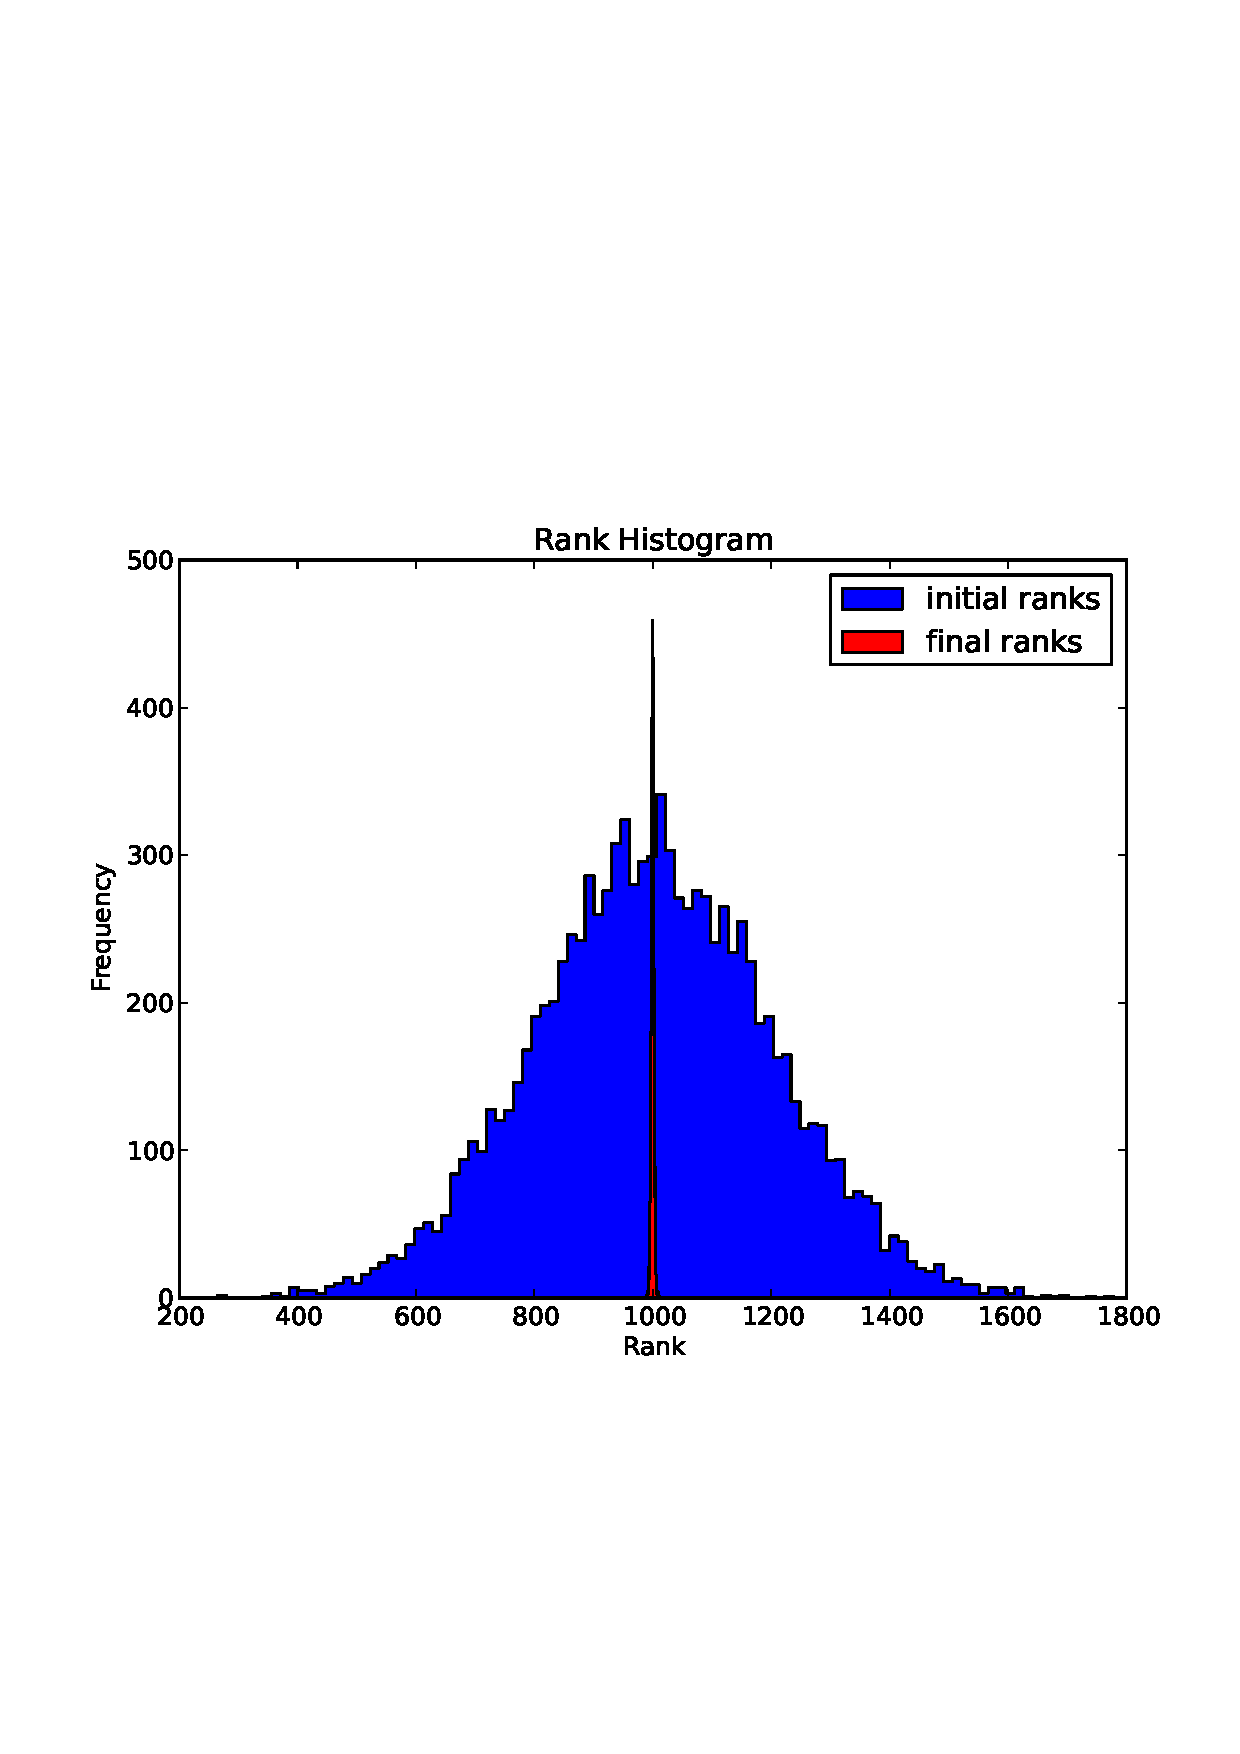
\includegraphics[width=15cm]{./images/sameAbilitiesRanks.pdf}
\end{center}
\caption{Rank histogram of initial ranks and final ranks for runners with no intrinsic ability. Initial $\mu=1000$ and $\sigma=200$, final $\mu=1000$ and $\sigma=2$; 30000 races in total. Note: bin widths are different for the two histograms.}
\label{fig:sameAbilitiesRanks}
\end{figure}\\
%\begin{figure}[h]     
%	\begin{center}
%    	\includegraphics[width=15cm]{./images/sameAbilitiesRanksStds.eps}
%	\end{center}
%	\caption{Standard deviation of means against race count for runners with no intrinsic ability.}
%	\label{fig:sameAbilitiesRanksStds}
%\end{figure}
Next, the 90\% cutoff rule was applied. It was observed that the rule produced a large drift (156 points) of the mean to the left, i.e. in the negative direction (see Fig \ref{fig:meanDrift}). The drift levels off as standard deviation decreases due to increasing sampling. The underlying cause was identified to be giving points to runners that were beyond the cutoff point. Removing the longest 10\% of run times for calculations of \emph{MT}, \emph{ST}, \emph{MP} and \emph{ST} while still giving points to the excluded runners creates a bias towards the lower scores. The mean run time is artificially lowered which leads to the excluded players receiving an inappropriately lower score which in turn leads to the whole rank distribution to drift to the left over time. Applying the same cutoff rule but this time not giving points to the excluded produced the same results as in Figure \ref{fig:sameAbilitiesRanks}.
%The decrease levels off as the standard deviation of the scores becomes smaller.
\begin{figure}[h]     
    \begin{center}                        
        \includegraphics[width=15cm]{./images/meanDrift.pdf}
	\end{center}
	\caption{Mean of scores against race count for runners with no intrinsic ability. Initial $\mu=1000$ and $\sigma=200$. The 90\% cutoff rule is applied. Error bars show standard deviation.}
	\label{fig:meanDrift}
\end{figure}\\
Runners with differing intrinsic abilities (see section \ref{sec:method} for implementation details) were put through the system next. To present the comparison between the runners' innate abilities and the rank assigned to them by the system, plots of these two quantities against each other are used. For a successful ranking attempt it is expected to see a straight line with a negative slope (higher mean run time corresponds to lower skill). If the runners make no mistakes, the system was found to correctly identify runners' abilities. Both Gaussian and constant initialization produced the correct plot showing that the system identified runners' intrinsic abilities correctly. However, with constant initialization some data (about 3\%) have a comparatively high standard deviation(see Fig \ref{fig:diffAbilitiesNoErrorConstantInit}). Examining these data points revealed that they usually have one race early on that produced a distant outlier, probably by putting them in a poorly matched race. Rerunning the simulation with the previously estimated ranks as the new initial ranks removed all outliers and produced consistent, small standard deviations. It is interesting that this effect did not arise when the system was initialized with Gaussian ranks. This was probably caused by initial "smoothing" of \emph{SP} so that very good runs did not earn an unreasonably high amount of points. These results inspire confidence that the code is correct.
%\begin{figure}[h]     
%    \begin{center}                        
%        \includegraphics[width=15cm]{./images/diffAbilitiesNoErrorNormalInit.png}
%	\end{center}
%	\caption{Mean of awarded scores plotted against mean run time(ability). Initial ranks were distributed from a Gaussian with $\mu=1000$ and $\sigma=200$. Final ranks have $\mu=1006$ and $\sigma=199$. Error bars show standard deviation, standard errors are too small to see.}
%	\label{fig:diffAbilitiesNoErrorNormalInit}
%\end{figure}
\begin{figure}[h]     
    \begin{center}                        
        \includegraphics[width=15cm]{./images/diffAbilitiesNoErrorConstantInit.png}
	\end{center}
	\caption{Mean of awarded scores plotted against mean run time. Initial ranks were all 1000. Final ranks have $\mu=1000$ and $\sigma=38$; 30000 races in total. Error bars show standard deviation, standard errors are too small to see. Points with high standard deviation represent about 3\% of the data.}
	\label{fig:diffAbilitiesNoErrorConstantInit}
\end{figure}\\
Adding in running mistakes, i.e. increasing noise, makes it more difficult to distinguish runners. The rank-ability plot bulges out and data points have high standard deviation (Fig \ref{fig:doubleFigure}a). Still, the general linear shape is retained so runners with significantly different abilities are correctly ranked with respect to each other. Increasing the number of races improves the ordering of runners, as one might expect, but the noise remains (Fig \ref{fig:doubleFigure}b). Interestingly, if the initial ranks were set to correctly reflect the runners' abilities, the rank-ability plot still bulged out as before.\\
%thus the initial conditions do not have a lasting effect on the final rankings
%Giving each runner a different capacity for making mistakes had little effect, the overall impact evens out.\\ 
Rerunning the same data multiple times while keeping the total number of races the same did not improve runner rank estimation. This can be explained by noting that generating unique races creates new information and thus improves the estimate of the mean. It was noted that the standard deviation of ranks would shrink when rerunning the same sequence of races multiple times. To explore this effect, runners with no mistakes were looped 10 times with 5000 races each loop. The mean and standard deviation of scores leveled off at 1000 and 38 respectively while the mean of standard deviations of individual racers' scores went to 0. The mean and individual deviations thus behaved correctly. It is unclear why the rank deviation went to 38 rather than 100 which was the standard deviation of the abilities but at least it was correctly identified that all runners are not the same.\\
To continue, runners with error making capability were run through 10 loops of 5000 races each as well. The mean of ranks remained at 1000 but both rank standard deviation and individual standard deviations approached 0. To examine this, the scores were rebased after every run except the last one to have mean 1000 and standard deviation 200. Now the standard deviation of ranks went to 90 and that of individual scores to 85, but increasing the number of races in each loop made these fall further. This indicates that all rebasing does is reset the initial standard deviation which then falls to where it intends to be. Different settings showed similar results.\\
It is unclear what exactly is causing the shrinking distribution. It seems to echo the Central Limit Theorem which, for a simple case like averaging coin tosses, would predict that the mean of averages would converge to a sharp peak. This, however, does not fully explain (i) why the case with no mistakes levels off a $\sigma=38$ instead of the standard distribution of the abilities(100) and (ii) why introducing even a small mistake propensity makes the distribution of scores shrink. Still, the rank-ability plots do not change qualitatively so the ordering of players, which is the ultimate goal, is not impeded. For practical reasons, though, it is desirable to rebase scores between reruns as doing so when the standard deviation falls very low can be difficult due to division by a very small number.
%In this case, however, the intermediate distributions of points being drawn from
\begin{figure}[h]     
    \begin{center} 
    	\begin{subfigure}{0.49\textwidth}                       
        	\includegraphics[width=\textwidth]{./images/diffAbilities10errorsGaussConstantInit3k.png}
        	\caption{3k races}
        \end{subfigure}
%        \begin{subfigure}{0.3\textwidth}                       
%        	\includegraphics[width=\textwidth]{./images/diffAbilities10errorsGaussConstantInit30k.png}
%        \end{subfigure}
        \begin{subfigure}{0.49\textwidth}                       
        	\includegraphics[width=\textwidth]{./images/diffAbilities10errorsGaussConstantInit100k.png}
        	\caption{100k races}
        \end{subfigure}
	\end{center}
	\caption{Mean of awarded scores plotted against mean run time for 2 different numbers of total races. Initial ranks were distributed from a Gaussian with $\mu=1000$ and $\sigma=200$. Final ranks have (a) $\mu=1000$ and $\sigma=92$ and (b) $\mu=1000$ and $\sigma=34$. Error bars show standard deviation, standard errors are too small to see.}
	\label{fig:doubleFigure}
\end{figure}\\
%
\FloatBarrier
\subsection{Data analysis results}
To get an idea of what the rank distribution should look like, raw race time data was analyzed. For every race time its distance in standard deviations from the mean of that particular race was calculated. The resulting distribution can be seen in Figure \ref{fig:timeDeviationDistribution}. It has a tail on the negative side which corresponds to race times that are larger than the mean. This is intuitive as achieving a very fast run is difficult while there is essentially no limit to how slow a race can be done. It is reasonable to expect that the rank distribution would have a similar shape.\\
Taking some of the observations from simulated data, a first look at the real Orienteering data was performed. The 90\% cutoff rule was not applied as it causes the distribution to drift significantly over time. Another concern with real data is poor sampling of some individuals. In the simulations runners were entered into races at random so with enough total races everyone was sampled well. In reality people have different levels of motivation, some participate frequently while others give up after one race. Both would be entered into the database. Thus in the final rank distribution only racers that have participated in 6 or more events were included. This choice was made arbitrarily to match the the fact that published scores are often the means of a runners' best 6 scores. Figure \ref{fig:simpleRealData} shows the resulting rank distributions. The data was initialized from a Gaussian an was run through twice to reduce the effect of initialization. The ranks display the same tail as the time deviation data as hoped. The fall on the right side is not as fast as that of the the time data. This could be due to only taking better sampled people into account who could be expected to perform better overall than the average due to practice.\\
Unfortunately, the shrinking of the distribution problem persisted here as with the simulated data. Repeated runs through the data caused the standard deviation of scores to fall each rerun without an obvious non-zero lower limit. Rebasing the scores between runs did not appear to improve the situation. This remains an unresolved problem and properties of convergence are unclear. Nevertheless, similarity between the time deviation and rank distributions and the earlier results from simulated data provide evidence that the people are still ranked as correctly as possible given limited data.\\
\begin{figure}[h]     
    \begin{center}                        
        \includegraphics[width=15cm]{./images/timeDeviationDistribution.pdf}
	\end{center}
	\caption{Distribution of all run time deviations obtained from real data. $\mu=0$ and $\sigma=1$. Negative deviation corresponds to race times that are larger than the mean.}
	\label{fig:timeDeviationDistribution}
\end{figure}
\begin{figure}[h]     
    \begin{center}                        
        \includegraphics[width=15cm]{./images/simpleRealData.pdf}
	\end{center}
	\caption{Rank histogram for real data with 2 different. Initial ranks were Gaussian with $\mu=1000$ and $\sigma=200$. The data was run through twice. Only people who participated in 6 or more races are shown. Final ranks have (a) $\mu=1000$ and $\sigma=55$. The black vertical line marks the mean.}
	\label{fig:simpleRealData}
\end{figure}
%In both cases the distributions have tails on the low rank side as expected. Constant initialization produces a smoother distribution than Gaussian initialization but it also produces distant outliers. Similarly as before, these runners were found to have a particularly low or high first few scores that biased their mean score. However, rerunning the the data again with the improved initial scores did not remove these outliers as was the case for simulated data. This suggests that the bad scores are based on actually outlying run times. To address this, a Gaussian cutoff rule was applied that ignores run times more than 2$\sigma$ outside the mean. Applying this rule and 2 runs through the data removed the high point outlier but the low ones remained. The outliers on the low end kept changing so it appears that there truly are some poor runners that belong there. However, the outlier at the top was the same person and it was observed that none of their runs were eliminated by the cutoff, but the initial high score disappeared still. Thus it can be concluded that the high outlier was caused by someone else's anomalous run time.
%\begin{figure}[H!]     
%    \begin{center} 
%    	\begin{subfigure}{0.49\textwidth}                       
%        	\includegraphics[width=\textwidth]{./images/realFirstLookConstant.pdf}
%        	\caption{•}
%        \end{subfigure}
%        \begin{subfigure}{0.49\textwidth}                       
%        	\includegraphics[width=\textwidth]{./images/realFirstLookNormal.pdf}
%        	\caption{•}
%        \end{subfigure}
%	\end{center}
%	
%	\caption{Rank histogram for real data with 2 different initialization types: (a) all 1000, (b) Gaussian with $\mu=1000$ and $\sigma=200$. Final ranks have (a) $\mu=1000$ and $\sigma=11$ and (b) $\mu=999$ and $\sigma=72$. The black vertical line marks the mean.}
%	\label{fig:firstLook}
%\end{figure}
%Next, the number of reruns were increased to 10. It was observed that the mean would drift linearly to the left. The Gaussian cutoff rule should be more careful than the 90\% rule in cutting out legitimate data. It then appears that the deeper cause of the drift is cutting out data from calculations of MT, ST, MP and SP while still assigning points to all racers. Repeating the run but this time not giving points to the outliers removed the drift previously observed.\\
%Another observed issue was the shrinking of the standard deviation of all ranks. This was accompanied by a small and decreasing drift of the mean to the right (previously it was to the left). If the system is trying to reach a steady state, the decrease of standard deviation means that any changes to rank also become smaller. Thus a lower limit on SP was imposed.
%[forgot to talk about max individual stds! those level off. individual rank changes also seem to level off. [without lower SP limit everything still falls to the floor]] [need to talk about the convergence, ie max/avg rank change] 